\chapter{Introducción a ROS\protect}

ROS, (Robot Operating System) es una herramienta para la creación de aplicaciones en robótica cuyo objetivo es promover el reuso de código de diferentes autores y para diferentes aplicaciones. Qué es ROS exactamente, cuál es su finalidad, para qué sirve y quiénes lo usan actualmente son preguntas que se responderan en esta sección\footnote{Este capítulo está basado en la documentación de ROS en http://wiki.ros.org/ROS/introduction}.

\section{¿Qué es ROS?}

ROS es un “meta-sistema operativo” de código libre que provee diferentes servicios que se esperarían de un sistema operativo, como abstracción de hardware, control de dispositivos en bajo nivel, funciones que se usan comúnmente, comunicación de procesos mediante mensajes y administración por paquetes. Bajo la licencia BSD es de libre uso, modificación y comercialización.

También incluye herramientas y librerías que permiten obtener, construir, escribir y ejecutar programas entre varios computadores. ROS es similar en algunas cosas con otros frameworks usados en robótica, tales como Player, Orocos, Yarp, Orca, Microsoft Robotics Studio, entre otros. ROS no es un framework en tiempo real, aunque sí es posible integrarlo con código en tiempo real, por ejemplo el robot PR2 de Willow Garage usa un sistema que se encarga de transportar mensajes en tiempo real. Incluso se ha integrado con el toolkit de tiempo real de OROCOS.


\section{Objetivos de ROS}

El objetivo de ROS no es ser un framework con las mejores características, en vez de esto, el objetivo principal de ROS es permitir el reuso de código en la investigación y el desarrollo de la robótica. ROS es un framework distribuido de procesos (llamados nodos) que permiten ser diseñados y acoplados de una manera sencilla en tiempo de ejecución. Estos nodos son organizados en paquetes, con lo que pueden ser fácilmente compartidos y distribuidos. ROS también tiene un sistema de repositorios que permiten la colaboración y distribución del código. Con este diseño, desde el sistema de archivos hasta la comunidad, se independiza el desarrollo y la implementación. Otros sub-objetivos en pro de cumplir con el  principal ideal son:

\begin{itemize}
\item Ser un sistema ligero y sencillo, integrable con otros frameworks
\item Desarrollo de librerías agnósticas
\item Independiente del lenguaje (Python, C++, Lisp, Java, Lua)
\item Fácil de probar
\item Escalable
\end{itemize}


\section{¿Qué contiene ROS?}

Entre el conjunto de librerías y herramientas que contiene ROS, cabe destacar su integración con software de procesamiento de imágenes como OpenCV\footnote{Open Source Computer Vision (http://opencv.org/)} y para el procesamiento de nubes de puntos como PCL\footnote{Point Cloud Library (http://pointclouds.org/)}. ROS también se integra con plataformas de simulación 2D como Stage\footnote{Stage Robot Simulator (http://rtv.github.io/Stage/)} y simulación 3D como Gazebo\footnote{Gazebo Simulator (http://gazebosim.org/)}.


Incluido en ROS se encuentra RVIZ que es una herramienta de visualización 3D que permite integrar información de sensores, modelos de robots y otros datos en una sola vista y también permite interactuar con esta visualización.

También ROS incluye rqt, un framework para desarrollo de interfaces gráficas basadas en QT. Estas interfaces son desarrolladas en forma de plugins, permitiendo que se puedan ejecutar individualmente u organizadas en una misma ventana. Estos plugin se pueden usar para la visualización de variables, gráficos, monitoreo de mensajes, nodos, entre otras cosas.

Otras utilidades que posee ROS son las herramientas de consola, que son un conjunto de comandos que sirven, entre otras cosas, para la navegación entre archivos y paquetes de ROS, ejecución de aplicaciones, creación de paquetes, etc.


\section{¿Por qué usar ROS?}

El desarrollo en robótica se sustenta en otros subcampos como navegación, percepción, planeación, razonamiento, entre otros. Debido a la amplitud de estos temas, la experiencia necesaria para programar un robot va más allá de la capacidad de una sola persona. Por esto se hace necesario simplificar la integración de diferente software de diferentes orígenes.

Además la robótica es un problema de integración de sistemas complejos y requiere un conjunto de herramientas para manejar esta complejidad. También es necesario que todos sus componentes puedan comunicarse entre sí de una manera eficiente ya que estos operan en el mundo real. ROS ofrece enfoques para cada uno de estos desafíos.

A Continuación se presentan algunas ventajas y desventajas del uso de ROS[6]
\begin{description}

\item{Ventajas} \hfill \\
\begin{itemize}

\item Gran cantidad de material desarrollado para robótica.
\item Hay una gran comunidad activa con interés en ROS.
\item Además de robótica, hay otros campos incluidos como ingeniería de software, colaboración en el desarrollo, modelos de código abierto, etc.
\item Accesible para todos, no solo expertos en ciencias de la computación.
\item Sirve de contexto para muchos sub-problemas de la robótica, así se puede observar como todo funciona en conjunto
\item Es una buena herramienta para problemas de M.Sc y Ph.D y es usado activamente en investigación
\item Amplio soporte de hardware (y creciendo).
\item Amplio soporte para simulación.
\item El reuso de código hace que lo que se demoraba hace unos años 3 meses, hoy toma un día.

\end{itemize}

\item{Desventajas} \hfill \\

\begin{itemize}

\item La curva de aprendizaje, especialmente para personas no relacionadas con las ciencias de la computación. Es un framework muy grande y puede ser aterrador. También puede ser difícil encontrar las cosas que se necesitan.
\item Linux, línea de comandos, multiterminal, multiproceso, distribuido, asíncrono. Puede ser más aterrador.
\item Gran cantidad de material desarrollado para robótica. Cuidado con los instructores perezosos, esto puede ser una desventaja.
\item Poco material dirigido al entorno universitario (Por ahora).
\item Falta de una comunidad cohesiva de educadores de ROS (Por ahora).

\end{itemize}
\end{description}

\section{Ejemplos del uso de ROS}

Debido a que ROS fue concebido como una herramienta para realizar aplicaciones en el campo de la robótica, su uso se ha extendido en todas las áreas y escenarios concernientes a esta. Se usa tanto en manipuladores como en plataformas móviles. En universidades y entornos académicos, ya sea para enseñanza o investigación y también en la industria. Incluso se creó el proyecto ROS Industrial\footnote{ROS Industrial (http://rosindustrial.org/)} como una extensión de ROS para aplicaciones industriales.

ROS también es un sistema multiplataforma; se ha usado con robots humanoides como NAO, plataformas para investigación como el PR2, robots industriales como Baxter, vehículos como los robots Pioneer, Kuka o Turtle Bot; e incluso plataformas educativas como el Lego Mindstorm NXT y la computadora Raspberry Pi. Algunas de estas plataformas se muestran en la figura \ref{robots}.


\begin{figure}[!ht]
\centering
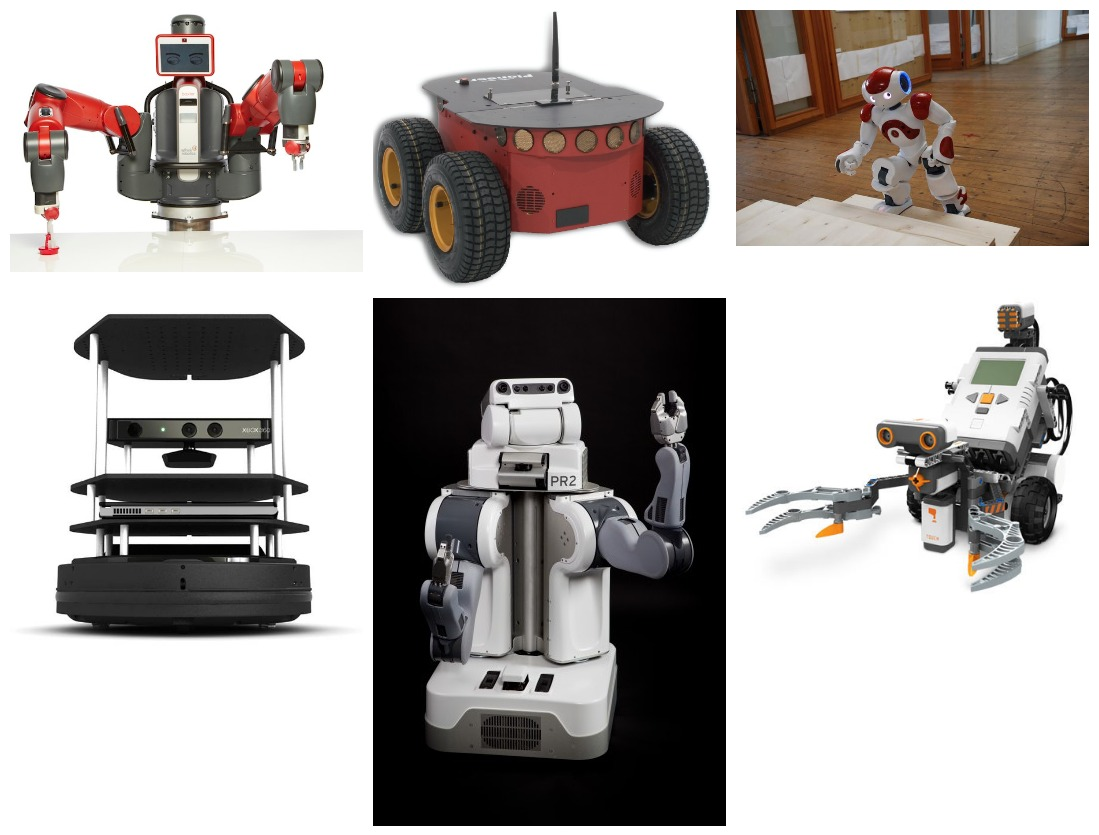
\includegraphics[scale=0.25]{img/robots.jpg}
\caption{Algunas plataformas en las que se usa ROS. Desde arriba a la izquierda: Baxter, Pioneer AT, NAO, TurtleBot 2, PR2, Lego Mindstorm NXT}
\label{robots}
\end{figure} 
